
\de{ĐỀ THI HỌC KỲ I NĂM HỌC 2022-2023}{THPT Nguyễn Tất Thành}



%%=====Bài 1
\begin{bt}%[0T3Y1-4]%[Dự án đề kiểm tra HK1 22-23-Nhật Thiện]%[THPT Nguyễn Tất Thành]
	Cho hàm số $y=f(x)$ có đồ thị như hình vẽ. Dựa vào đồ thị, tìm tập xác định, tập giá trị và các khoảng đồng biến, nghịch biến của hàm số.(Hs không cần vẽ hình)
	\begin{center}
		\begin{tikzpicture}[>=stealth,line join=round,line cap=round,font=\footnotesize,scale=0.75]
			\tikzset{declare function ={x1=-7.5;x2=6.5;y1=-3.5;y2=4.5;}}
			\draw[opacity=.2,gray] (x1,y1)grid (x2,y2);
			\draw[->,thick](x1,0)--(x2,0)node[above]{$x$};
			\draw[->,thick](0,y1)--(0,y2)node[left]{$y$};
			\draw (0,0)circle(1.2pt)node[below left]{$O$};
			\draw (-6,-3)coordinate (A)--(-2,3)coordinate (B)to [out=-80,in=160](0,-1)coordinate (C)--(5,4)coordinate (D)node[below=1]{$y=f(x)$};
			\foreach \i/\goc in {-2/-90,-6/-90,5/-90,1/-80}{
				\draw (\i, 0) node[shift={(\goc:2mm)}]{$\i$};	
			}
			\foreach \i/\goc in {-3/0,-1/-0,3/0,4/0}{
				\draw (0,\i) node[shift={(\goc:2mm)}]{$\i$};	
			}
			\foreach \point in {A,B,C,D}{
				\draw[fill=black](\point)circle(1.2pt);
			}
		\end{tikzpicture}
	\end{center}
	\dapso{Tập xác định $\mathscr{D}=[-6;5]$, tập giá trị $\mathscr{T}=[-3;4]$, hàm số đồng biến trên $(-6;-2)$ và $(0;5)$, hàm số nghịch biến trên $(-2;0)$.}
	\loigiai{
		Quan sát hình vẽ, tập xác định $\mathscr{D}=[-6;5]$, tập giá trị $\mathscr{T}=[-3;4]$, hàm số đồng biến trên $(-6;-2)$ và $(0;5)$, hàm số nghịch biến trên $(-2;0)$.
	}
\end{bt}

%%=====Bài 2
\begin{bt}%[0T3Y1-3]%[Dự án đề kiểm tra HK1 22-23-Nhật Thiện]%[THPT Nguyễn Tất Thành]
	Vẽ đồ thị của hàm số $y=x^2+2 x-3$. Tìm tập giá trị và các khoảng đồng biến, nghịch biến của hàm số.\\
	\dapso{Đồ thị hàm số
		\begin{tikzpicture}[>=stealth,line join=round,line cap=round,font=\footnotesize,scale=.5]
			
			\tikzset{declare function ={x1=-3.5;x2=2.5;y1=-4.5;y2=2.5;}}
			\tikzset{declare function={a=1;b=2;c=-3; f(\x)=a*(\x)^2+b*(\x)+c;}}
			\clip (x1-.5,y1-.5)rectangle(x2+.5,y2+.5);
			\draw[opacity=.2,gray] (x1,y1)grid (x2,y2);
			\draw[->,thick](x1,0)--(x2,0)node[above]{$x$};
			\draw[->,thick](0,y1)--(0,y2)node[left]{$y$};
			\draw (0,0)circle(1.2pt)node[below left]{$O$};
			\draw[samples=1000,domain=-3.5:1.5] plot(\x,{f(\x)});
			\foreach \i/\goc in {-3/-135,-1/90,1/-60}{
				\draw (\i, 0) node[shift={(\goc:2.5mm)}]{$\i$};	
			}
			\foreach \i/\goc in {-4/0,-3/0}{
				\draw (0,\i) node[shift={(\goc:2.5mm)}]{$\i$};	
			}
			\draw[dashed] (-1,0)|-(0,-4);
		\end{tikzpicture}\\
		Tập giá trị $T=[-4;+\infty)$, hàm số nghịch biến trên $(-\infty;-1)$ và nghịch biến trên $(-1;+\infty)$.}
	\loigiai{
		Hàm số $y=x^2+2x-3$ ($a=1$, $b=2$, $c=-3$).\\
		Đỉnh $S$ của đồ thị hàm số có tọa độ $x_S=-\dfrac{b}{2a}=-1$, $y_S=(-1)^2+2(-1)-3=-4$.\\
		Suy ra tập giá trị $T=[-4;+\infty)$.\\
		Vì hàm số bậc hai có $a=1>0$ nên ta có bảng biến thiên sau
\begin{center}
		
\begin{tikzpicture}[scale=1, font=\footnotesize, line join=round, line cap=round, >=stealth]
			\tkzTabInit[nocadre=false,lgt=1.2,espcl=2.5,deltacl=0.6]
			{$x$ /0.6,$y$ /2}
			{$-\infty$,$-1$,$+\infty$}
			\tkzTabVar{+/$+\infty$,-/$-4$,+/$+\infty$}
		\end{tikzpicture}
\end{center}
		Hàm số đồng biến trên khoảng $(-1;+\infty)$ và nghịch biến trên khoảng $(-\infty;-1)$.\\
		Bảng giá trị
		\begin{center}
		\begin{tabular}{c|c|c|c|c|c}
			$x$ & $-3$ & $-2$ & $-1$ & $0$ & $1$\\
			\hline
			$y$ & $0$ & $-3$ & $-4$ & $-3$ & $0$
		\end{tabular}
\end{center}
		Đồ thị hàm số
		\begin{center}
		\begin{tikzpicture}[>=stealth,line join=round,line cap=round,font=\footnotesize,scale=.5]
			
			\tikzset{declare function ={x1=-3.5;x2=2.5;y1=-4.5;y2=2.5;}}
			\tikzset{declare function={a=1;b=2;c=-3; f(\x)=a*(\x)^2+b*(\x)+c;}}
			\clip (x1-.5,y1-.5)rectangle(x2+.5,y2+.5);
			\draw[opacity=.2,gray] (x1,y1)grid (x2,y2);
			\draw[->,thick](x1,0)--(x2,0)node[above]{$x$};
			\draw[->,thick](0,y1)--(0,y2)node[left]{$y$};
			\draw (0,0)circle(1.2pt)node[below left]{$O$};
			\draw[samples=1000,domain=-3.5:1.5] plot(\x,{f(\x)});
			\foreach \i/\goc in {-3/-135,-2/90,-1/90,1/-60}{
				\draw (\i, 0) node[shift={(\goc:2.5mm)}]{$\i$};	
			}
			\foreach \i/\goc in {-4/0,-3/0}{
				\draw (0,\i) node[shift={(\goc:2.5mm)}]{$\i$};	
			}
			\draw[dashed] (-1,0)|-(0,-4)  (-2,0)|-(0,-3);
		\end{tikzpicture}

\end{center}
	}
\end{bt}

%%=====Bài 3
\begin{bt}%[0T3B1-3]%[Dự án đề kiểm tra HK1 22-23-Nhật Thiện]%[THPT Nguyễn Tất Thành]
	Tìm các số $a$, $b$, $c$, biết đồ thị hàm số $y=a x^2+b x+c$ qua $A(0;-3)$ và có đỉnh $S(-2; 1)$.
	\dapso{$a=-1$; $b=-4$; $c=-3$}
	\loigiai{
		Đồ thị hàm số qua $A(0;-3)$ suy ra $-3=a\cdot 0^2+b\cdot 0+c$ hay $c=-3$.\\
		Đồ thị hàm số có đỉnh $S(-2;1)$ suy ra $\heva{&-\dfrac{b}{2a}=-2\\&1=a(-2)^2+b(-2)+c}\Leftrightarrow \heva{&4a-b=0\\&4a-2b+c=1.}$\\
		Ta có hệ phương trình
		$$\heva{&4a-b=0\\&4a-2b-3=1}\Leftrightarrow \heva{&4a-b=0\\&4a-2b=4}\Leftrightarrow \heva{&a=-1\\&b=-4.}$$
		Vậy $a=-1$; $b=-4$; $c=-3$.
	}
\end{bt}



%%=====Bài 4
\begin{bt}%[0T2K2-2]%[Dự án đề kiểm tra HKI NH22-23- Thành Đức Trung]%[THPT Nguyễn Tất Thành - Hồ Chí Minh]
Một công ty sản xuất hai loại sơn nội thất và sơn ngoài trời. Nguyên liệu để sản xuất gồm hai loại A, B với trữ lượng là $12$ tấn và $8$ tấn tương ứng. Để sản xuất $1$ tấn sơn nội thất cần $5$ tấn nguyên liệu A và $1$ tấn nguyên liệu B. Để sản xuất $1$ tấn sơn ngoài trời cần $2$ tấn nguyên liệu A và $2$ tấn nguyên liệu B. Qua điều tra thị trường, công ty thấy nhu cầu sơn nội thất không hơn sơn ngoài trời quá $1$ tấn. Giá bán $1$ tấn sơn nội thất là $2000$ USD, giá bán $1$ tấn sơn ngoài trời là $3000$ USD. Hỏi cần sản xuất mỗi loại sơn bao nhiêu tấn đề có doanh thu lớn nhất?
%\dapso{Để đạt doanh thu lớn nhất cần sản xuất $1$ tấn sơn nội thất và $3{,5}$ tấn sơn ngoài trời.}
\loigiai
{
Gọi $x$ là lượng sơn nội thất cần sản xuất, $y$ là lượng sơn ngoài trời cần sản suất. \\
Theo giả thiết ta có $\heva{ & x\geqslant0 \\ & y\geqslant0 \\ & 5x+2y\leqslant12 \\ & x+2y\leqslant8 \\ & x-y\leqslant1.}$ \hfill $(1)$ \\
Doanh thu là giá trị của hàm số $f(x;y)=2x+3y$ (nghìn USD). \\
Biểu diễn miền nghiệm của $(1)$ lên mặt phẳng tọa độ $Oxy$
\begin{center}
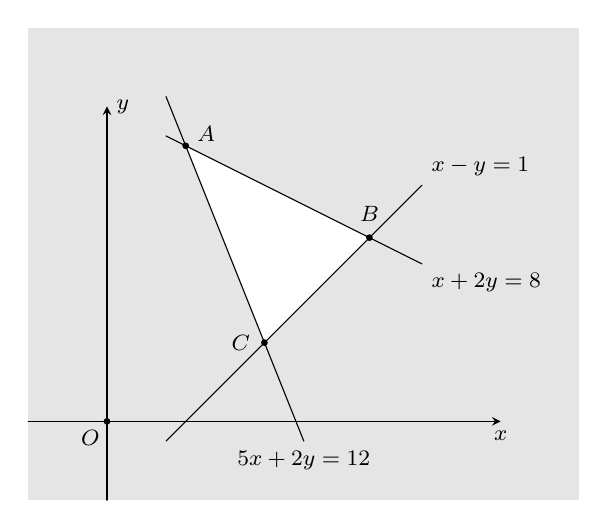
\begin{tikzpicture}[line cap=round, line join=round, >=stealth, scale=1, font=\footnotesize]
\fill[black!10](-1,-1)rectangle(6,5);
\path
(1,7/2)coordinate(A)
(10/3,7/3)coordinate(B)
(2,1)coordinate(C)
(0,0)coordinate(O)
;
\fill[white](A)--(B)--(C)--cycle;
\draw[->](-1,0)--(5,0) node[below]{$x$};
\draw[->](0,-1)--(0,4)node[right]{$y$};
\draw[smooth, domain=0.75:2.5]plot(\x,{(12-5*(\x))/2})node[below]{$5x+2y=12$};
\draw[smooth, domain=0.75:4]plot(\x,{((\x)-1})node[above right]{$x-y=1$};
\draw[smooth, domain=0.75:4]plot(\x,{(8-(\x))/2})node[below right]{$x+2y=8$};
\foreach\x/\y in {A/30,B/90,C/180,O/-135} \draw[fill=black] (\x) circle (1pt)+(\y:0.3) node{$\x$};
\end{tikzpicture}	
\end{center}
Miền nghiệm của $(1)$ là tam giác $ABC$ (và phần bên trong của nó) với $A\left(1;\dfrac{7}{2}\right)$, $B\left(\dfrac{10}{3};\dfrac{7}{3}\right)$, $C(2;1)$. \\
Ta có $f(A)=\dfrac{25}{2}$, $f(B)=\dfrac{41}{3}$, $f(C)=7$. \\
Vậy cần sản xuất $1$ tấn sơn nội thất và $3{,5}$ tấn sơn ngoài trời thì doanh thu cao nhất.
}
\end{bt}

%%=====Bài 5
\begin{bt}%[0T5G4-4]%[Dự án đề kiểm tra HKI NH22-23- Thành Đức Trung]%[THPT Nguyễn Tất Thành - Hồ Chí Minh]
Cho hình vuông $ABCD$ tâm $I$, $AD=3$. Gọi $G$ là trọng tâm $\triangle BCD$.
\begin{enumerate}
\item Tính $\left|\overrightarrow{AD}+\overrightarrow{DC}\right|$; $\left|\overrightarrow{GB}+\overrightarrow{GD}\right|$; $\overrightarrow{IA}\cdot\overrightarrow{GD}$; $\overrightarrow{AD}\cdot\overrightarrow{DB}$.
\item Chứng minh rằng $\overrightarrow{AD}-\overrightarrow{BG}-2\overrightarrow{CG}=6\overrightarrow{IG}$.
\item Tìm tất cả các điểm $M$ thỏa mãn điều kiện $\overrightarrow{GI}\cdot\overrightarrow{IM}=\dfrac{3}{4}$.
\end{enumerate}
%\dapso
%{
%\begin{enumerate}
%\item $|\overrightarrow{A D}+\overrightarrow{D C}|=3\sqrt{2}$; $|\overrightarrow{G B}+\overrightarrow{G D}|=\sqrt{2}$; $\overrightarrow{I A} \cdot \overrightarrow{G D} =1$; $\overrightarrow{A D} \cdot \overrightarrow{D B}=-9$.
%\item[c)]  $M$ chạy trên đường thẳng qua $E$ $\left(E\in IG\text{ và }\overrightarrow{GI}\cdot \overrightarrow{IE}=\dfrac{3}{4}\right)$, vuông góc với $IG$.
%\end{enumerate}
%}
\loigiai
{
\begin{enumerate}
\item
\immini
{
\begin{itemize}
\item Ta có $\left|\overrightarrow{AD}+\overrightarrow{DC}\right|=\left|\overrightarrow{AC}\right|=AC=\sqrt{AD^2+DC^2}=3\sqrt{2}$.
\item Ta có $\overrightarrow{GB}+\overrightarrow{GC}+\overrightarrow{GD}=\overrightarrow{0} \Rightarrow \overrightarrow{GB}+\overrightarrow{GD}=-\overrightarrow{GC}$, \\
suy ra $\left|\overrightarrow{GB}+\overrightarrow{GD}\right|=\left|-\overrightarrow{GC}\right|=GC=\dfrac{2}{3}CI=\dfrac{1}{3}AC=\sqrt{2}$.
\item Ta có $\overrightarrow{IA}\cdot\overrightarrow{GD}=\overrightarrow{IA}\cdot\left(\overrightarrow{GI}+\overrightarrow{ID}\right)=\overrightarrow{IA}\cdot\overrightarrow{GI}+\overrightarrow{IA}\cdot\overrightarrow{ID}$. \\
Ta có $\overrightarrow{IA}\cdot\overrightarrow{GI}=-\overrightarrow{IA}\cdot\overrightarrow{IG}=-IA\cdot IG\cdot\cos\left(\overrightarrow{IA},\overrightarrow{IG}\right)$. \\
Ta có $\heva{ & IA=\dfrac{1}{2}AC=\dfrac{3\sqrt{2}}{2} \\ & IG=\dfrac{1}{3}IC=\dfrac{1}{6}AC=\dfrac{\sqrt{2}}{2} \\ & \cos\left(\overrightarrow{IA},\overrightarrow{IG}\right)=\cos180^{\circ}=-1} \Rightarrow \overrightarrow{IA}\cdot\overrightarrow{GI}=\dfrac{3}{2}$. \\
Ta có $\overrightarrow{IA}\cdot\overrightarrow{ID}=0$ vì $IA\perp ID$. \\
Suy ra $\overrightarrow{IA}\cdot\overrightarrow{GD}=\dfrac{3}{2}$.
\item Ta có $\overrightarrow{AD}\cdot\overrightarrow{DB}=-\overrightarrow{DA}\cdot\overrightarrow{DB}=-DA\cdot DB\cdot\cos\left(\overrightarrow{DA},\overrightarrow{DB}\right)$. \\
Ta có $\heva{ & DA=3 \\ & DB=AC=3\sqrt{2} \\ & \cos\left(\overrightarrow{DA},\overrightarrow{DB}\right)=\cos45^{\circ}=\dfrac{\sqrt{2}}{2}} \Rightarrow \overrightarrow{AD}\cdot\overrightarrow{DB}=-9$.
\end{itemize}
}
{
\begin{tikzpicture}[line cap=round, line join=round, font=\footnotesize, >=stealth, scale=1]
\path
(0,0)coordinate(A)
(3,0)coordinate(B)
(3,3)coordinate(C)
(0,3)coordinate(D)
($(B)!0.5!(D)$)coordinate(I)
($(C)!2/3!(I)$)coordinate(G)
($(A)!0.5!(D)$)coordinate(E)
($(A)!0.5!(B)$)coordinate(F)
($(E)!0.5!(F)$)coordinate(X)
($2*(E)-(X)$)coordinate(Y)
($2*(F)-(X)$)coordinate(Z)
;
\draw
(A)--(B)--(C)--(D)--(A)--(C)
(G)--(B)--(D)--(G)--(E)--(I)
(Z)node[below]{$d$}--(Y)
;
\foreach\x/\y in {A/-135, B/-90, C/45, D/180, I/-90, G/90, E/-135} \draw[fill=black] (\x) circle (1pt)+(\y:0.3) node{$\x$};
\end{tikzpicture}	
}
\item
Vì $G$ là trọng tâm tam giác $BCD$ nên $\dfrac{GC}{CI}=\dfrac{2}{3} \Rightarrow \dfrac{GC}{AC}=\dfrac{1}{3} \Rightarrow \dfrac{GC}{AG}=\dfrac{1}{2} \Rightarrow AG=2GC$. \\
Ta có
$$\begin{aligned}
& \ \overrightarrow{AD}-\overrightarrow{BG}-2\overrightarrow{CG}=6\overrightarrow{IG} \Leftrightarrow \overrightarrow{GD}-\overrightarrow{GA}+\overrightarrow{GB}+2\overrightarrow{GC}=3\overrightarrow{GC} \\
\Leftrightarrow & \ \overrightarrow{GB}+\overrightarrow{GC}+\overrightarrow{GD}+\overrightarrow{AG}=2\overrightarrow{GC} \Leftrightarrow \overrightarrow{AG}=2\overrightarrow{GC}\text{: luôn đúng}.
\end{aligned}$$
\item Ta có $\overrightarrow{GI}\cdot\overrightarrow{IM}=\dfrac{3}{4} \Leftrightarrow \overrightarrow{IG}\cdot\overrightarrow{IM}=-\dfrac{3}{4}$. \hfill $(1)$ \\
Gọi $E$ là trung điểm $AD$, ta có
$$(1) \Leftrightarrow \overrightarrow{IG}\cdot\left(\overrightarrow{IE}+\overrightarrow{EM}\right)=-\dfrac{3}{4} \Leftrightarrow \overrightarrow{IG}\cdot\overrightarrow{IE}+\overrightarrow{IG}\cdot\overrightarrow{EM}=-\dfrac{3}{4}. \quad (2)$$
Ta có $\overrightarrow{IG}\cdot\overrightarrow{IE}=IG\cdot IE\cdot\cos\left(\overrightarrow{IG},\overrightarrow{IE}\right)$. \\
Ta có $\heva{ & IG=\dfrac{\sqrt{2}}{2} \\ & IE=\dfrac{1}{2}AB=\dfrac{3}{2} \\ & \cos\left(\overrightarrow{IG},\overrightarrow{IE}\right)=\cos\widehat{GIE}=135^{\circ}=-\dfrac{\sqrt{2}}{2}} \Rightarrow \overrightarrow{IG}\cdot\overrightarrow{IE}=-\dfrac{3}{4}$. \\
Khi đó $(2) \Leftrightarrow \overrightarrow{IG}\cdot\overrightarrow{EM}=0$. \\
Vậy tất cả các điểm $M$ là đường thẳng $d$ đi qua $E$ và vuông góc với $IG$.
\end{enumerate}
}
\end{bt}